\section{Chaining}
This chapter concerns some of the central methods for bounding random processes $(X_t)$. We'll go over concepts 
such as chaining, VC theory, generic chaining methods, and bounds such as Talagrand's inequality and Chevet's 
inequality. We'll apply these to concepts such as Monto Carlo integration, empirical processes, and statistical 
learning theory.



% ----------8.1----------
\subsection{Dudley Inequality}
For a general Gaussian process $(X_t)_{t \in T}$, Sudakove inequality (\cref{thm:7.4.1}) gives a \textit{lower} 
bound on 
\[ \mathbb{E}\left[ \sup_{t \in T}X_t \right] \]
in terms of the metric entropy pf $T$. Now we'll go for an upper bound. Moreover, we generalize from Gaussian 
processes to subgaussian processes as well.

\begin{definition}[]
\label{def:8.1.1}
A random process $(X_t)_{t \in T}$ on a metric space $(T, d)$ has \underline{subgaussian increments} if there 
exists $K > 0$ such that 
\[ \lVert X_t - X_s \rVert_{\psi_2} \leq Kd(t, s) \text{ for all } t, s \in T. \]
\end{definition}

\begin{example}[Gaussian processes]
\label{ex:8.1.2}
Let $(X_t)_{t \in T}$ be a Gaussian process on some set $T$. It naturally defines a \textit{canonical metric} 
on $T$: 
\[ d(t, s) := \lVert X_t - X_s \rVert_{L^2}, \ t, s \in T, \]
as we explained earlier. With respect to this metric, $(X_t)_{t \in T}$ clearly has subgaussian increments, 
with some absolute constant $K$.
\end{example}

Here is another (trivial) example: Any random process can be made to have subgaussian increments by defining 
the metric as $d(t, s) := \lVert X_t - X_s \rVert_{\psi_2}$.

Now we give a bound on a general subgaussian random process in terms of the metric entropy:

\begin{theorem}[Dudley's integral inequality]
\label{thm:8.1.3}
Let $(X_t){t \in T}$ be a mean-zero random process on a metric space $(T, d)$ with subgaussian increments as in 
\cref{def:8.1.1}. Then 
\[ \mathbb{E}\left[ \sup_{t \in T}X_t \right] \leq CK \int_{0}^{\infty} 
\sqrt{\log_{}{\mathcal{N}(T, d, \varepsilon)}} \ d \varepsilon. \]
\end{theorem}

Before going to the proof's let's compare Dudley's inequality with Sudakov's inequality (\cref{thm:7.4.1}), 
which for Gaussian processes, says:
\[ \mathbb{E}\left[ \sup_{t \in T}X_t \right] \geq c \sup_{\varepsilon > 0}\varepsilon 
\sqrt{\log_{}{\mathcal{N}(T, d, \varepsilon)}}. \]
Figure 8.1 below shows both bounds: 
\begin{center}
	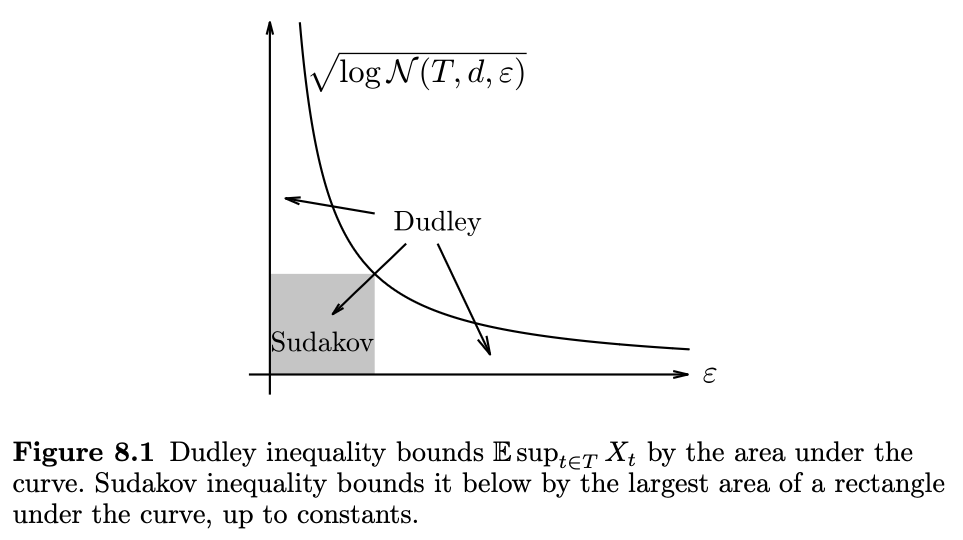
\includegraphics[width=0.8\textwidth]{Chapter 8/fig8-1.png}
\end{center}
There is a clear gap between the two bounds, and it turns out that metric entropy alone cannot close it - we 
will explore this later.

Dudley's inequality hints that $\mathbb{E}\left[ \sup_{t \in T}X_t \right]$ is a \textit{multiscale} quantity 
- to bound it, we need to look at $T$ across all scales $\varepsilon$. That's exactly how the proof works! But 
let's prove a discrete version using syadic scaled $\varepsilon = 2^{-k}$ like a Riemann sum, then move to the 
continuous version later.

\begin{theorem}[Discrete Dudley's inequality]
\label{thm:8.1.4}
Let $(X_t)_{t \in T}$ be a mean-zero random process on a metric space $(T, d)$ with subgaussian increments as 
from earlier. Then 
\[ \mathbb{E}\left[ \sup_{t \in T}X_t \right] \leq CK \sum_{k \in \mathbb{Z}}^{}2^{-k} 
\sqrt{\log_{}{\mathcal{N}(T, d, \varepsilon)}}. \]
\end{theorem}

The proof uses a technique called \textit{chaining}. It is a multi-scaled version of the $\varepsilon$-net 
argument that we did in \cref{thm:4.4.3} and \cref{thm:7.6.1}. In the $\varepsilon$-net argument, we approximate 
$T$ by an $\varepsilon$-net $\mathcal{N}$ so every point $t \in T$ is close to some $\pi(t) \in \mathcal{N}$, 
with $d(t, \pi(t)) \leq \varepsilon$. Then the increment condition gives 
\[ \lVert X_t - X_{\pi(t)} \rVert_{\psi_2} \leq K \varepsilon. \]
This leads to 
\[ \mathbb{E}\left[ \sup_{t \in T}X_t \right] \leq \mathbb{E}\left[ \sup_{t \in T}X_{\pi(t)} \right] 
+ \mathbb{E}\left[ \sup_{t \in T}(X_t - X_{\pi(t)}) \right]. \]
We can handle the first term via union bound over $|\mathcal{N}| = \mathcal{N}(T, d, \varepsilon)$ points 
$\pi(t)$. However, the second term is unclear (if we were to use union bound) since there is both $t$ and 
$\pi(t)$ in the supremum. To fix this, we don't stop at one net, but choose smaller and smaller $\varepsilon$ 
to get better approximations $\pi_1(t), \pi_2(t), \dots$ to $t$ with finer nets. This is the idea behind 
\textit{chaining}.

\begin{proof}[Proof of \cref{thm:8.1.4}]
\textbf{Step 1: Chaining setup.} Without loss of generality, we may assume that $K = 1$ (because of $C$) and 
$T$ is finite (\cref{rmk:7.2.1}). Define the dyadic scale 
\[ \varepsilon_k = 2^{-k}, \ k \in \mathbb{Z} \]
and choose $\varepsilon_k$-nets $T_k$ of $T$ so that 
\[ |T_k| = \mathcal{N}(T, d, \varepsilon_k). \]
Only a part of the dyadic scale will be needed. Since $T$ is finite, there exists a small enough number 
$\kappa \in \mathbb{Z}$ (defining the coarsest net) and a large enough number $K \in \mathbb{Z}$ (defining the 
finest net), such that 
\[ T_{\kappa} = \{t_0\} \text{ for some } t_0 \in T, \ T_K = T. \]
For a point $t \in T$, let $\pi_l(t)$ denote a closest point in $T_k$, so we have 
\[ d(t, \pi_k(t)) \leq \varepsilon_k. \]
Since $\mathbb{E}\left[ X_{t_0} \right] = 0$ by assumption, 
\[ \mathbb{E}\left[ \sup_{x \in T}X_t \right] = \mathbb{E}\left[ \sup_{x \in T}(X_t - X_{t_0}) \right]. \]
Let's write $X_t - X_{t_0}$ as a telescoping sum, walking from $t_0$ to $t$ along a chain (aha!) of points 
$\pi_k(t)$ that mark progressively finer approximations of $t$:
\[ X_t - X_{t_0} = (X_{\pi_{\kappa}(t)} - X_{t_0}) + (X_{\pi_{\kappa + 1}(t)} - X_{\pi_{\kappa}(t)}) 
+ \cdots + (X_t - X_{\pi_{K}(t)}), \]
see Figure 8.2 below for an illustration.
\begin{center}
    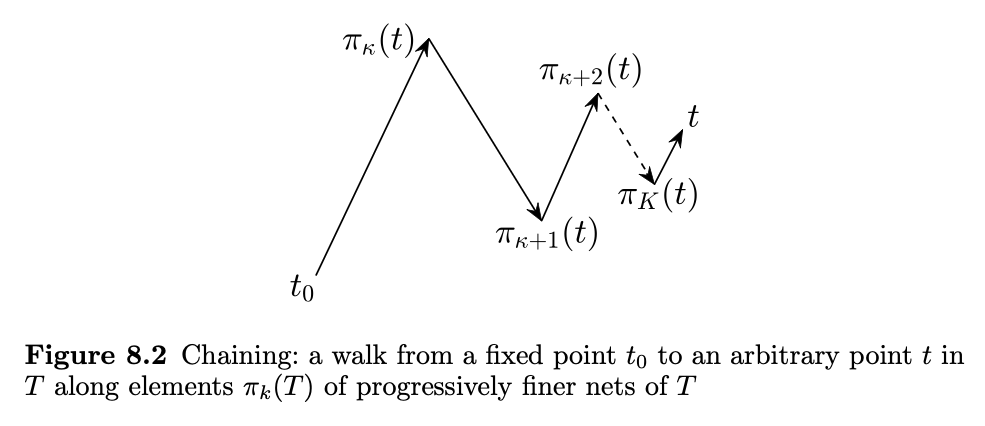
\includegraphics[width=0.8\textwidth]{Chapter 8/fig8-2.png}
\end{center}
The first and last terms of this sum are zero by our definition earlier, so we have 
\[ X_t - X_{t_0} = \sum_{k = \kappa + 1}^{K} (X_{\pi_k(t)} - X_{\pi_{k - 1}(t)}). \]
Since the supremum of the sum is bounded by the sum of the suprema, we get 
\[ \mathbb{E}\left[ \sup_{t \in T}(X_t - X_{t_0}) \right] \leq 
\sum_{k = \kappa + 1}^{K} \mathbb{E}\left[ \sup_{t \in T}(X_{\pi_k(t)} - X_{\pi_{k - 1}(t)}) \right]. \]

\textbf{Step 2: Controlling the increments.} In the equation above, it looks like we are taking the supremum 
over all of $T$ in each summand, but really it is over the smaller set of pairs $(\pi_k(t), \pi_{k - 1}(t))$. 
The number of such pairs is 
\[ |T_k| \cdot |T_{k - 1}| = |T_k|^2, \]
A number that we can control via covering numbers from above. Moreover, for a fixed $t$, we can bound the 
increments in step 1 like this: 
\begin{align*}
	\lVert X_{\pi_k(t)} - X_{\pi_{k - 1}(t)} \rVert_{\psi_2} 
	&\leq d(\pi_k(t), \pi_{k - 1}(t)) \quad \text{(By \cref{def:8.1.1})} \\ 
	&\leq d(\pi_k(t), t) + d(t, \pi_{k - 1}(t)) \quad \text{(By triangle inequality)} \\
	&\leq \varepsilon_k + \varepsilon_{k - 1} \quad \text{(By definition of )} \pi_k(t) \\
	&\leq 2 \varepsilon_{k - 1}.
\end{align*}
Recall from \cref{prop:2.7.6} that the expected maximum of $N$ subgaussian random variables is at most 
$CL \sqrt{\log_{}{N}}$, where $L$ is the largest $\psi_2$ norm. We can use this to bound each term: 
\[ \mathbb{E}\left[ \sup_{t \in T}(X_{\pi_k(t)} - X_{\pi_{k - 1}(t)}) \right] 
\leq C \varepsilon_{k - 1} \sqrt{\log_{}{|T_k|}}. \]

\textbf{Step 3: Summing up the increments.} We have shown that 
\[ \mathbb{E}\left[ \sup_{t \in T}(X_t - X_{t_0}) \right] 
\leq C \sum_{k = \kappa + 1}^{K} \varepsilon_{k - 1} \sqrt{\log_{}{|T_k|}}. \]
Now plug in the values $\varepsilon_k = 2^{-k}$ and the bounds on $|T_k|$, we get 
\[ \mathbb{E}\left[ \sup_{t \in T}(X_t - X_{t_0}) \right] 
\leq C_1 \sum_{k = \kappa + 1}^{K} 2^{-k} \sqrt{\log_{}{\mathcal{N}(T, d, 2^{-k})}}. \]
Hence the theorem is proved.
\end{proof}

Let's now go for the proof for the integral form of Dudley's inequality.

\begin{proof}[Proof of Dudley's integral inequality (\cref{thm:8.1.3})]
To convert the sum from the discrete form into an integral, we express $2^{-k}$ as 
$2 \int_{2^{-k-1}}^{2^{-k}}  \ d \varepsilon$. Then 
\[ \sum_{k \in \mathbb{Z}}^{} 2^{-k} \sqrt{\log_{}{\mathcal{N}(T, d, 2^{-k})}} = 
2 \sum_{k \in \mathbb{Z}}^{} \int_{2^{-k-1}}^{2^{-k}} \sqrt{\log_{}{\mathcal{N}(T, d, 2^{-k})}} \ 
d \varepsilon. \]
Within the limits of the integral, $2^{-k} \geq \varepsilon$, hence $\log_{}{\mathcal{N}(T, d, 2^{-k})} 
< \log_{}{\mathcal{N}(T, d, 2^{-k})}$ and the sum is bounded by 
\[ 2 \sum_{k \in \mathbb{Z}}^{} \int_{2^{-k-1}}^{2^{-k}} \sqrt{\log_{}{\mathcal{N}(T, d, \varepsilon)}} \ 
d \varepsilon = 2 \int_{0}^{\infty} \sqrt{\log_{}{\mathcal{N}(T, d, \varepsilon)}} \ d \varepsilon, \]
and the proof is complete.
\end{proof}

Actually, the discrete and integral Dudley inequalities are equivalent (Exercise 8.3).


\subsubsection{Variations and Examples}
\begin{remark}[Dudley's inequality: supremum of increments]
\label{rmk:8.1.5}
A quick look at the proof shows that chaining actually gives 
\[ \mathbb{E}\left[ \sup_{t \in T}|X_t - X_{t_0}| \right] \leq CK 
\int_{0}^{\infty} \sqrt{\log_{}{\mathcal{N}(T, d, \varepsilon)}} \ d \varepsilon \]
for any fixed $t \in T$. We can combine with the same bound for $X_s - X_{t_0}$, then use the triangle 
inequality to get 
\[ \mathbb{E}\left[ \sup_{t, s \in T}|X_t - X_s| \right] \leq CK 
\int_{0}^{\infty} \sqrt{\log_{}{\mathcal{N}(T, d, \varepsilon)}} \ d \varepsilon. \]
\end{remark}

\begin{remark}[Dudley's inequality: a high-probability bound]
\label{rmk:8.1.6}
Dudley's inequality gives only an expectation bound, but chaining actually gives a high-probability bouind. 
Assuming $T$ is finite (avoid measurability issues), for every $u \geq 0$, the bound 
\[ \sup_{t, s \in T} |X_t - X_s| \leq CK \left[ \int_{0}^{\infty} \sqrt{\log_{}{\mathcal{N}(T, d, \varepsilon)}} 
\ d \varepsilon + u \cdot \mathrm{diam}(T) \right] \]
holds with probability at least $1 - 2 \exp{(-u^2)}$ (Exercise 8.1). For Gaussian processes, this also follows 
directly from Gaussian concentration (Exercise 8.2).
\end{remark}

\begin{remark}[Limits of Dudley integral]
\label{rmk:8.1.7}
Even though the Dudley integral goes over $[0, \infty]$, we can cap it at the diameter of $T$, since for 
$\varepsilon > \mathrm{diam}(T)$, a single $\varepsilon$-ball covers $T$ and so 
\[ \mathcal{N}(T, d, \varepsilon) = 1 \implies \log_{}{\mathcal{N}(T, d, \varepsilon)} = 0. \]
Thus 
\[ \mathbb{E}\left[ \sup_{t \in T}X_t \right] \leq CK \int_{0}^{\mathrm{diam}(T)} 
\sqrt{\log_{}{\mathcal{N}(T, d, \varepsilon)}} \ d \varepsilon. \]
\end{remark}

If we apply Dudley's inequality for the canonical Gaussian process $\left\langle g, t \right\rangle$, just 
like we did with Sudakov's inequality in \cref{cor:7.4.2}, we get the following:

\begin{theorem}[Dudley's inequality in \texorpdfstring{$\mathbb{R}^n$}{}]
\label{thm:8.1.8}
The Gaussian width of any bounded set $Y \subset \mathbb{R}^n$ satisfies 
\[ w(T) \leq C \int_{0}^{\infty} \sqrt{\log_{}{\mathcal{N}(T, \varepsilon)}} \ d \varepsilon, \]
where $\mathcal{N}(T, \varepsilon)$ is the smallest number of Euclidean balls with radius $\varepsilon$ and 
centers in $T$ that cover $T$.
\end{theorem}

\begin{example}[Dudley's inequality is sharp for the Euclidean ball]
\label{ex:8.1.9}
Let's test Dudley's inequality for the unit Euclidean ball $T = B_2^n$. From \cref{cor:4.2.11}, 
\[ \mathcal{N}(B_2^n, \varepsilon) \begin{cases}
	\leq (3 / \varepsilon)^n &\text{ for } \varepsilon \in (0, 1], \\
	= 1 &\text{ for } \varepsilon > 1
\end{cases}. \]
Then 
\[ w(B_2^n) \lesssim \int_{0}^{1} \sqrt{n \log_{}{(3 / \varepsilon)}} \ d \varepsilon \lesssim \sqrt{n}. \]
This is in fact optimal: as we know from \cref{ex:7.5.6}, $w(B_2^n) \asymp \sqrt{n}$.
\end{example}

\begin{remark}[Dudley's inequality can be loose - but not too loose]
\label{rmk:8.1.10}
In general, Dudley integral can overestimate the Gaussian width. Here is a bad example: 
\[ T = \left\{ \frac{e_k}{\sqrt{1 + \log_{}{k}}}, \ k = 1, \dots, n \right\} \]
with $e_k$ being the standard basis in $\mathbb{R}^n$. From exercise 8.4, we can see that 
\[ w(T) = O(1) \text{ while } \int_{0}^{\infty} \sqrt{\log_{}{\mathcal{N}(T, d, \varepsilon)}} \ d \varepsilon 
\to \infty \]
as $n \to \infty$. However, the good news:
\begin{enumerate}
	\item Dudley equality is tight up to a logarithmic factor (Exercise 8.5);
	\item We will use chaining to remove that logarithmic factor in Section 8.5.
\end{enumerate}
\end{remark}


% ----------8.2----------
\subsection{Application: Empirical Processes}



% ----------8.3----------
\subsection{VC Dimension}
VC dimensions measures how complex a class of Boolean functions is, where a Boolean function is a map 
$f: \omega \to \{0, 1\}$ on some set $\omega$, and we are looking at some collection $\mathcal{F}$ of these.

\begin{definition}[]
\label{def:8.3.1}
A subset $\Lambda \subseteq \Omega$ is \underline{shattered} by a class of boolean functions $\mathcal{F}$ if, 
for any possible binary labeling $g: \Lambda \to \{0, 1\}$, there is some function $f \in \mathcal{F}$ that 
matches it on $\Lambda$. Formally, this means the restriction of $f$ onto $\Lambda$ is $g$, i.e. 
$f(x) = g(x) \text{ for all } x \in \Lambda$.

The \underline{Vapnik-Chervonenkis dimension (VC dimension)} of $\mathcal{F}$, denoted 
$\mathrm{vc}(\mathcal{F})$, is the largest cardinality of a subset $\Lambda \subseteq \Omega$ that is shattered. 
If there is no largest one, then $\mathrm{vc}(\mathcal{F}) = \infty$.
\end{definition}

Let's go through a few examples to make the definition clearer:

\begin{example}[Intervals]
\label{ex:8.3.2}
Let $\mathcal{F}$ consist of the indicators of all closed intervals in $\mathbb{R}$:
\[ \mathcal{F} = \left\{ \mathbf{1}_{[a, b]}: \ a, b \in \mathbb{R}, \ a \leq b \right\}. \]
We claim that 
\[ \mathrm{vc}(F) = 2. \]

We first show that $\mathrm{vc}(\mathcal{F}) \geq 2$ by finding a two-point set $\Lambda \subset \mathbb{R}$ 
that is shattered by $\mathcal{F}$. Take, for example, $\Lambda = 3, 5$. There are four possible binary 
labelings $g: \Lambda \to \{0, 1\}$ on this set, and each one can be obtained by restricting some interval 
indicator $f = \mathbf{1}_{[a, b]}$ ontp $\Lambda$. For example, $g(3) = 1, g(5) = 0$ comes from 
$f = \mathbf{1}_{[2, 4]}$. The other three cases are shown in Figure 8.5, so $\Lambda$ is indeed shattered by 
$\mathcal{F}$.

\begin{center}
    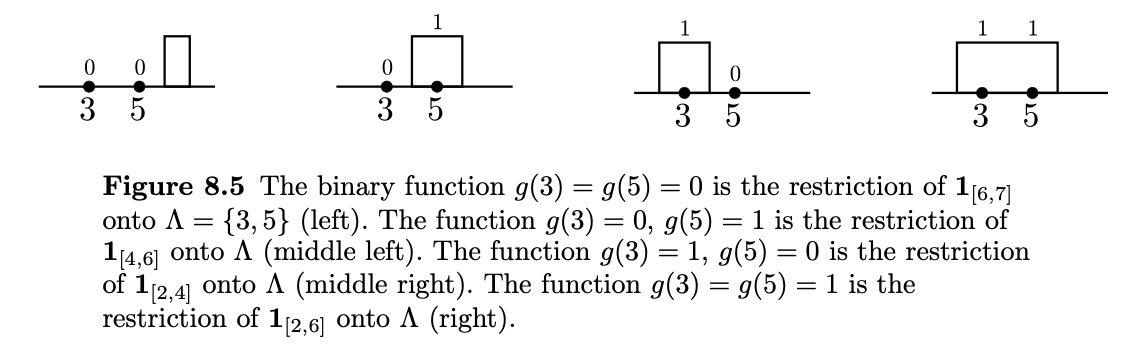
\includegraphics[width=0.8\textwidth]{Chapter 8/fig8-5.png}
\end{center}

To prove $\mathrm{vc}(\mathcal{F}) < 3$, we need to show that no three-point set $\Lambda = \{p, q, r\}$ can 
be shattered by $\mathcal{F}$. To see this, assume $p < q < r$ and consider the labeling $g(p) = 1, g(q) = 0, 
g(r) = 1$. Then $g$ cannot be a restriction of any indicator interval onto $\Lambda$ (it is not linearly 
seperable).
\end{example}



% ----------8.4----------
\subsection{Application: Statistical Learning Theory}



% ----------8.5----------
\subsection{Generic Chaining}



% ----------8.6----------
\subsection{Chevet Inequality}



